
\section{Основная часть}

    \subsection{Определение модели}

        Модель Hassell имеет следующую математическая запись:

        \[x_{t+1} = \frac{\alpha x_t^2}{(\beta + x_t)^6}\]

        где \(x_i\) --- количество особей в поколении с номером i. Параметр \(\alpha\) определяет скорость роста популяции, а параметр \(\beta\) определяет несущую способность окружающей среды.
    
    \subsection{Частный случай}
    
        Зафиксируем параметр \(\alpha = 1\). Параметр \(\beta\) изменяется в диапазоне \([0; 0.6]\). Также запишем уравнение в таком виде:

        \[x = \frac{\alpha x^2}{(\beta + x)^6}\]
    
        \[1 = \frac{\alpha x}{(\beta + x)^6}\]

        \[\alpha x = (\beta + x)^6\]

        Теперь можно построить графики функций \(y = \alpha x\) и \(y = (\beta + x)^6\). В зависимости от значений параметра \(\beta\) уравнение может иметь ноль, одну или две общие точки. На рисунках (\ref{mainTouch}), (\ref{mainIntersect}), (\ref{mainOver}) можно увидеть все возможные варианты.

        \begin{figure}[h!]
            \centering
            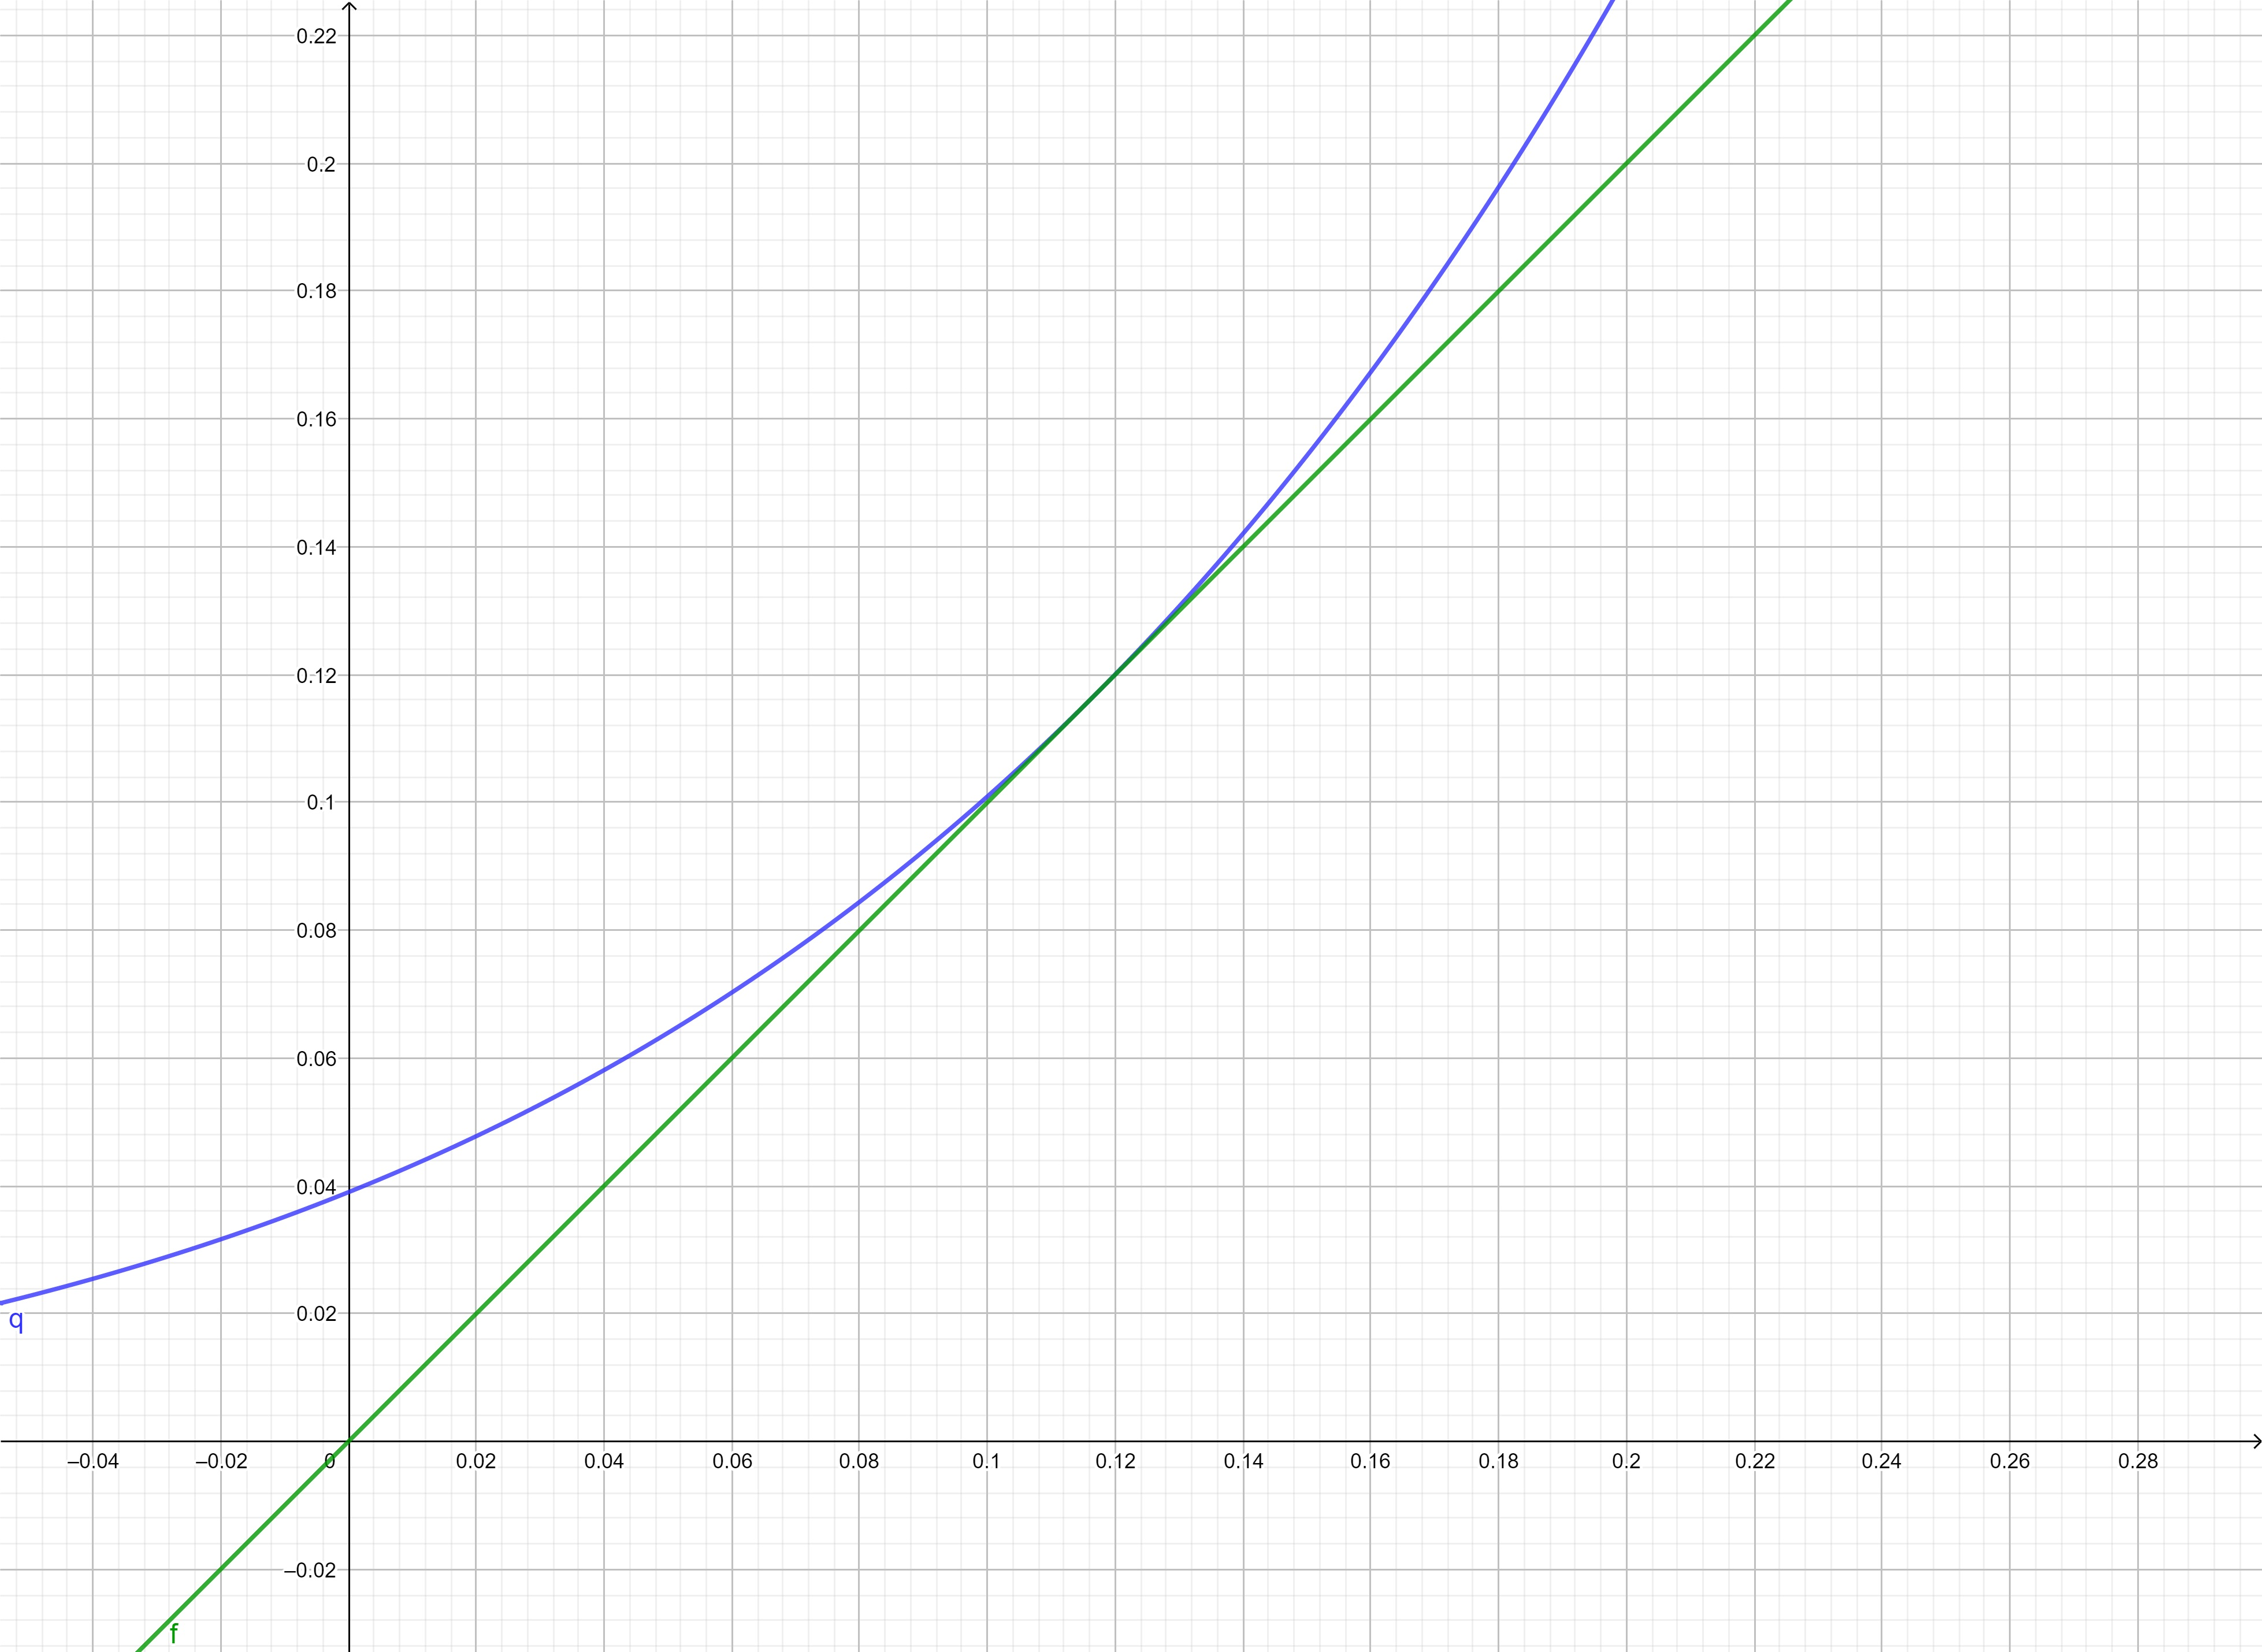
\includegraphics[width=0.8\textwidth]{images/main_touch.jpg}

            \caption{Синяя линия --- \(\frac{\alpha x^2}{(\beta + x)^6}\); Зеленая линия --- \(\frac{\alpha x^2}{(\beta + x)^6}; \beta \approx 0.582355932\). Два корня}
            \label{mainTouch}
        \end{figure}

        \begin{figure}[h!]
            \centering
            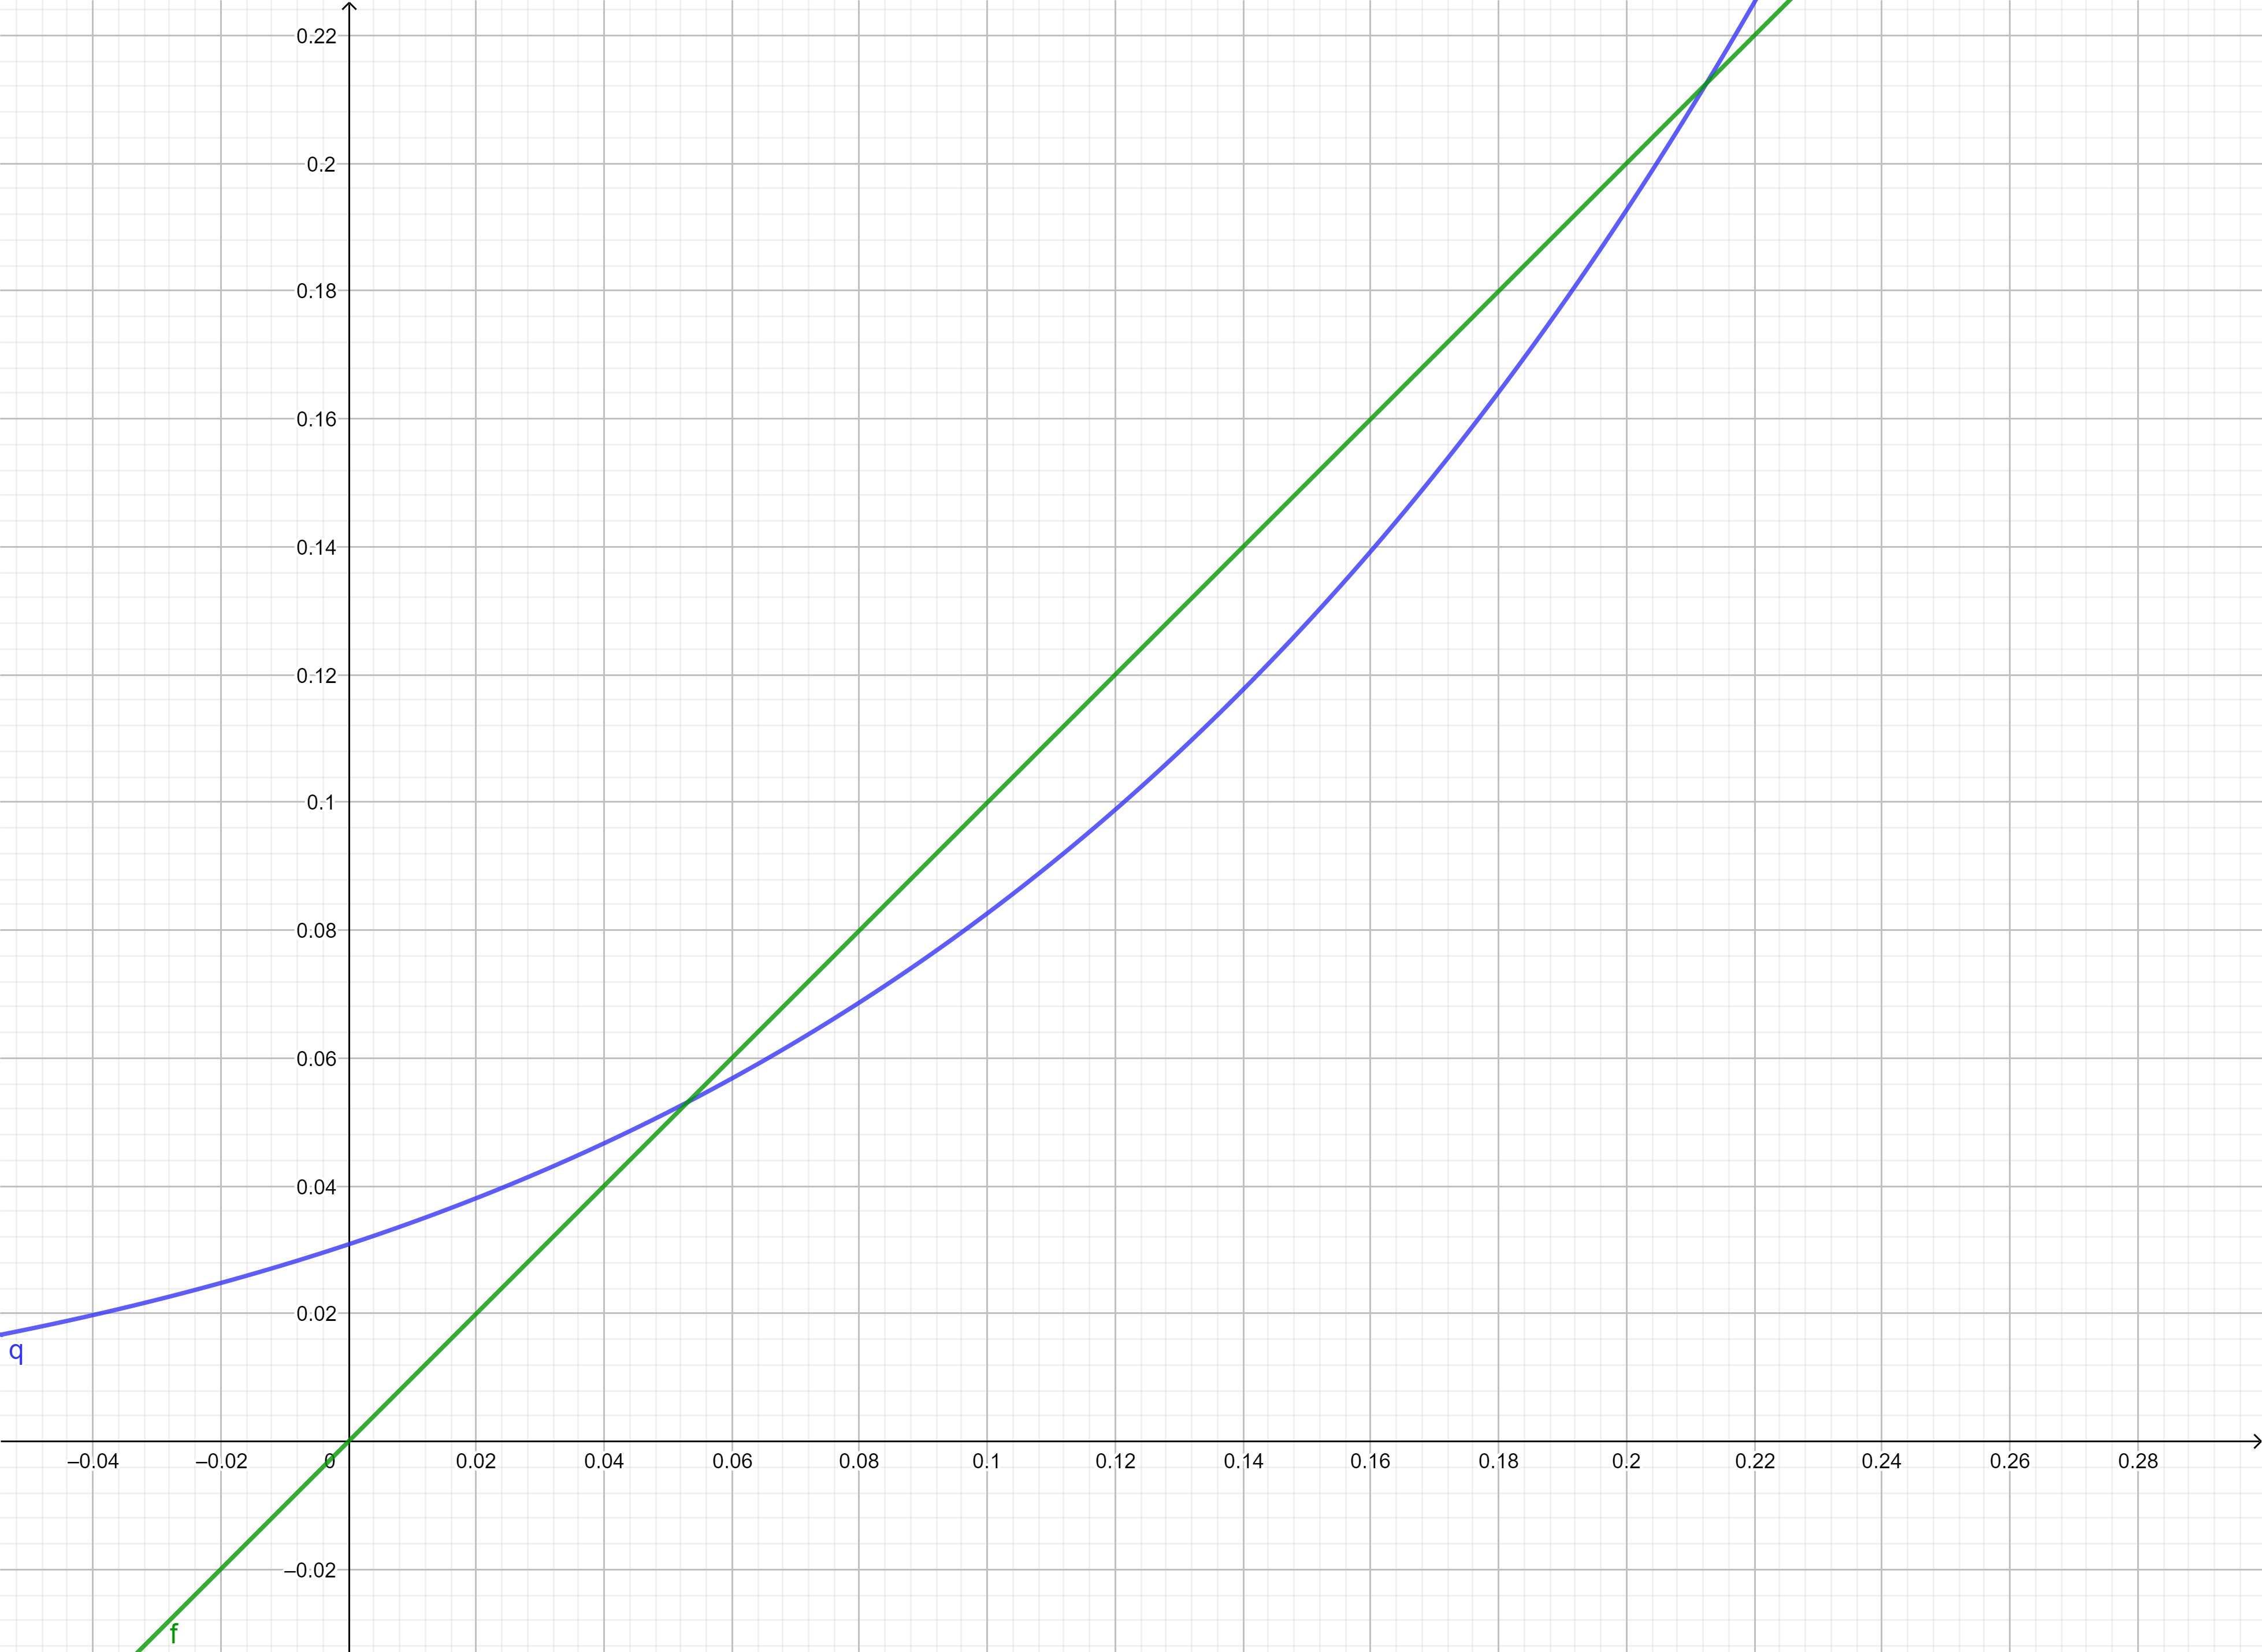
\includegraphics[width=0.8\textwidth]{images/main_intersect.jpg}

            \caption{Синяя линия --- \(\frac{\alpha x^2}{(\beta + x)^6}\); Зеленая линия --- \(\frac{\alpha x^2}{(\beta + x)^6}; \beta < 0.582355932\). Три корня}
            \label{mainIntersect}
        \end{figure}

        \begin{figure}[h!]
            \centering
            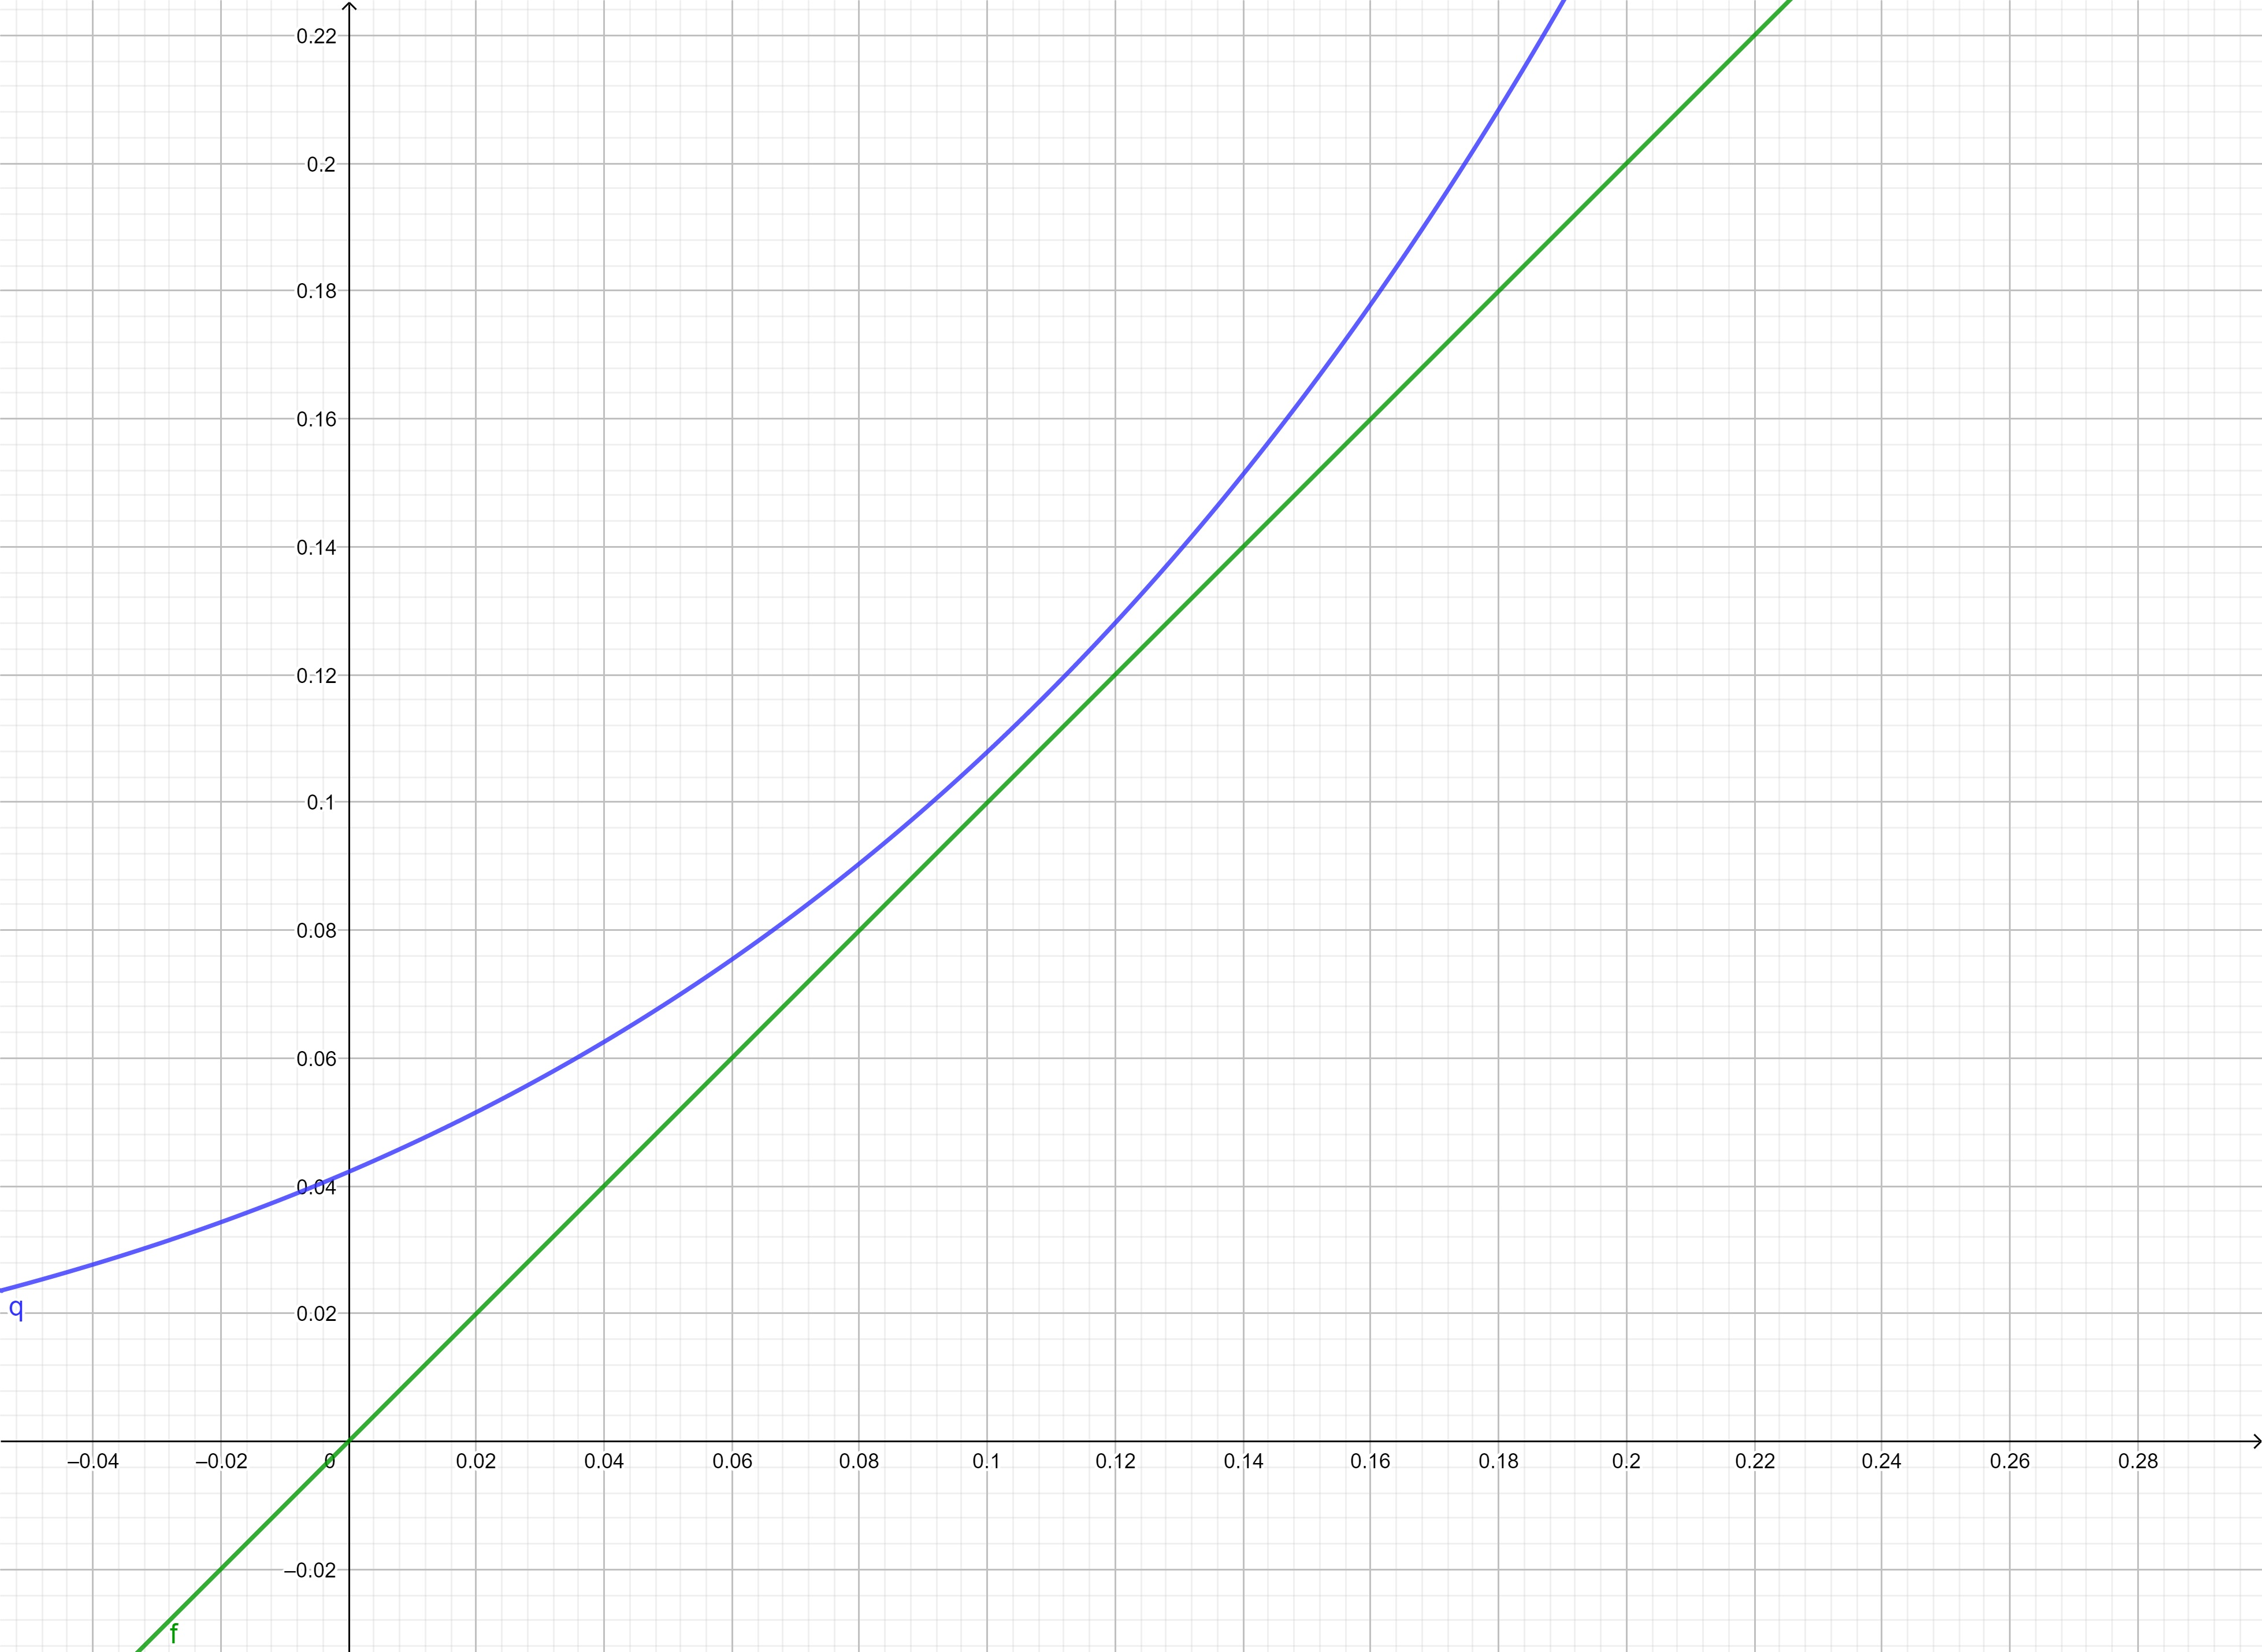
\includegraphics[width=0.8\textwidth]{images/main_over.jpg}

            \caption{Синяя линия --- \(\frac{\alpha x^2}{(\beta + x)^6}\); Зеленая линия --- \(\frac{\alpha x^2}{(\beta + x)^6}; \beta > 0.582355932\). Три корня}
            \label{mainOver}
        \end{figure}

        \par\noindent\rule{\textwidth}{0.4pt}

        Аналитически это уравнение не решается. Для нахождения корней будем использовать метод Ньютона.

        В зависимости от конкретных значений параметра \(\beta\) данное уравнение может иметь от одного до трех корней.
    
        *графики какие-нибудь*

        Для того, чтобы найти корни с помощью метода Ньютона рассмотрим уравнение 
    
        \[x - \frac{\alpha x^2}{(\beta + x)^6} = 0\]

        При \(\beta \approx 0.582355932\) уравнение имеет два корня: \(x_0 = 0\) и \(\bar{x}_1 \approx 0.116471186636\). При \(\beta < 0.582355932\) - три корня,а при \(\beta > 0.582355932\) - один корень \(x_0 = 0\).
    
        Корень == точке равновесия.

        Можно построить временные ряды.

        \begin{figure*}[h]
            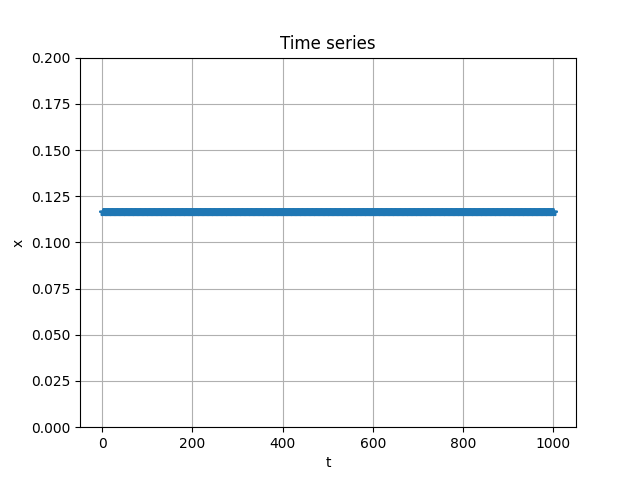
\includegraphics[scale=0.8]{Time_series_x_011647_b_0582355932}    
            \caption{Временной ряд при \(x_0 \approx 0.11647\) и \(\beta \approx 0.582355932\)}
        \end{figure*}

        Наверное, еще какие-нибудь ряды надо вставить\dots Только что надо показать на них?
